\documentclass[11pt, a4paper, onecolumn]{article}
\usepackage[a4paper,margin=1in,footskip=0.25in]{geometry}
 
\usepackage{graphicx}
\usepackage{enumerate}
\usepackage[utf8]{inputenc}
\usepackage{xcolor}
\usepackage{hyperref}
\usepackage{subfig}
\usepackage{floatrow}

\usepackage{amsmath}
\usepackage{amssymb}
\usepackage{arydshln}

\usepackage{tikz}
\usetikzlibrary{positioning,arrows,decorations.markings}

\newcommand{\tjzm}{$t$-$J^z$~model}
\newcommand{\Ket}[1]{\left\vert #1 \right\rangle}
\newcommand{\Bra}[1]{\left\langle #1 \right\vert}
\newcommand{\ket}[1]{\vert #1 \rangle}
\newcommand{\bra}[1]{\langle #1 \vert}
\newcommand{\abs}[1]{\left\vert #1 \right\vert}

\def\K{%
    \operatornamewithlimits{%
        \mathchoice{% * Display style
            \vcenter{\hbox{\huge $\mathcal{K}$}}%
        }{%           * Text style
            \vcenter{\hbox{\Large $\mathcal{K}$}}%
        }{%           * Script style
            \mathrm{\mathcal{K}}%
        }{%           * Script script style
            \mathrm{\mathcal{K}}%
        }
    }
}

\def\composition{\operatornamewithlimits{\circ}}

\providecommand{\newoperator}[3]{%
	\newcommand*{#1}{\mathop{#2}#3}}
\providecommand{\renewoperator}[3]{%
	\renewcommand*{#1}{\mathop{#2}#3}}
	
\newoperator{\srot}%
	{\mathrm{rot}}{\nolimits}

\newoperator{\ent}%
	{\mathrm{ent}}{\nolimits}
	
\renewoperator{\Re}%
	{\mathrm{Re}}{\nolimits}
	
\renewoperator{\Im}%
	{\mathrm{Im}}{\nolimits}	
	
\makeatletter
\providecommand*{\diff}%
	{\@ifnextchar^{\DIfF}{\DIfF^{}}}
	
\def\DIfF^#1{%
	\mathop{\mathrm{\mathstrut d}}%
	\nolimits^{#1}\gobblespace}
	
\def\gobblespace{%
	\futurelet\diffarg\opspace}
	
\def\opspace{%
	\let\DiffSpace\!%
		\ifx\diffarg(%
			\let\DiffSpace\relax
		\else
			\ifx\diffarg[%
				\let\DiffSpace\relax
			\else
				\ifx\diffarg\{%
					\let\DiffSpace\relax
				\fi\fi\fi\DiffSpace}
				
\providecommand*{\deriv}[3][]{%
	\frac{\diff^{#1}#2}{\diff #3^{#1}}}
\providecommand*{\pderiv}[3][]{%
	\frac{\partial^{#1}#2}%
		{\partial #3^{#1}}}
		
\newcommand{\mean}[1]{\langle#1\rangle}

\begin{document}

\section{From position states to rotational states}

Let us consider the $t$--$J^z$ Hamiltonian $H$ (in holon-magnon basis) and an empty (for holes and magnons) Bethe lattice with coordination $z=4$. Let denote this empty lattice as vacuum state $\ket{\varnothing}$. Next, let us choose a certain site in the Bethe lattice and refer to this site as the origin of the lattice by denoting it as $j=0$. Let us further create a hole in the origin of the lattice and let denote the resulting \textit{initial} state as $\ket{0}$,
\begin{equation}
	\ket{0} = h_{j=0}^\dag \ket{\varnothing}.
\end{equation} 
Let us consider two orthogonal states $\psi_1$ and $\psi_2$. We will say that $\psi_2$ is $n$-reachable from $\psi_1$ if $n$ is smallest positive integer such that $\bra{\psi_2}H^n\ket{\psi_1} \neq 0$. If such an integer does not exist, we will say that $\psi_2$ and $\psi_1$ are disconnected (or non-reachable from one another). Let us find all the states $n$-reachable from $\ket{0}$ for $n=1,2,3,\hdots$. We can do it by acting on $\ket{0}$ with $H^n$ for different values of $n$. 

Let's start with $n=1$.
\begin{equation}
	H\ket{0} = E_0 \ket{0} - t(\ket{1;0}+\ket{1;1}+\ket{1;2}+\ket{1;3}).
\end{equation}
In the above notation $\ket{n;d_1,...,d_n}$ is a \textit{position} state with $n$ magnons where the hole has moved through bonds in directions $d_1,...,d_n$ (without returning) in the given order (i.e. from $d_1$ to $d_n$). The condition for states to be $n$-reachable does not specify the basis. We could for example choose 4 position states,
\begin{equation}
	\ket{1;0}, \quad \ket{1;1}, \quad \ket{1;2}, \quad \ket{1;3}
\end{equation}
to describe the subspace of states 1-reachable from $\ket{0}$. But we could also mix them to get so-called \textit{rotational} states,
\begin{equation}
	\ket{1;m^{(1)}_4}_r = \frac{1}{\sqrt{4}}\sum_{d_1=0}^3 \exp\left(\frac{2 \pi i}{4}d_1 m^{(1)}_4\right)\ket{1;d_1},
\end{equation}
where $m^{(1)}_4 = 0,...,3$. The initial state in the rotational representation is simply $\ket{0}_r = \ket{0}$. It is straightforward to notice,
\begin{equation}
	_r\bra{1;m^{(1)}_4} H\ket{0} = -2t \delta_{0,m^{(1)}_4},
\end{equation}
which means only states with $0$ angular momentum are 1-reachable from $\ket{0}$. 

Let now move to $n=2$. States that are 2-reachable from $\ket{0}$ are the same as states 1-reachable from $\ket{1;d_1}$ after summing over $d_1$,
\begin{equation}
	H\ket{1;d_1} = E_1 \ket{1;d_1} - t(\ket{2;d_1,0}+\ket{2;d_1,1}+\ket{2;d_1,2}),
\end{equation}
which in total gives 12 states $\ket{2;d_1,d_2}$. Here again, we have the freedom of choice when it comes to the basis. The position states $\ket{2;d_1,d_2}$ are the simplest choice, but not the only one. We can for example introduce a mixed basis, where only the last move is considered to have a rotational description,
\begin{equation}
	\ket{2;d_1,m^{(2)}_3}_m = \frac{1}{\sqrt{3}}\sum_{d_2=0}^2 \exp\left(\frac{2 \pi i}{3}d_2 m^{(2)}_3\right)\ket{2;d_1,d_2}.
\end{equation}
Moreover, applying recursively the rotation to all the positional degrees of freedom, we arrive at the rotational states fully described by the two angular momenta, $\phi_1 = \frac{2\pi}{4}m^{(1)}_4$ and $\phi_2 = \frac{2\pi}{3}m^{(2)}_3$,
\begin{equation}
	\ket{2;m^{(1)}_4,m^{(2)}_3}_r = \frac{1}{\sqrt{12}}\sum_{d_1=0}^3 \sum_{d_2=0}^2 \exp\left(\frac{2 \pi i}{4}d_1 m^{(1)}_4\right) \exp\left(\frac{2 \pi i}{3}d_2 m^{(2)}_3\right)\ket{2;d_1,d_2}.
\end{equation}
And again, we can notice,
\begin{equation}
	_r\bra{2;m^{(1)}_4,m^{(2)}_3}H\ket{1;0}_r = -\sqrt{3}t \delta_{0,m^{(1)}_4} \delta_{0,m^{(2)}_3},
\end{equation}
which means only states with $m^{(1)}_4 = m^{(2)}_3 = 0$ are 2-reachable from $\ket{0}$. 

Let us now consider the general case of $n>1$. There are no surprises,
\begin{equation}
\begin{aligned}
	H\ket{n-1;d_1,...,d_{n-1}} &= E_{n-1} \ket{n-1;d_1,...,d_{n-1}} \\
	&- t(\ket{n;d_1,...,d_{n-1},0}+\ket{n;d_1,...,d_{n-1},1}+\ket{n;d_1,...,d_{n-1},2}),
\end{aligned}
\end{equation}
and the mixed basis can also be introduced,
\begin{equation}
	\ket{n;d_1,...,d_{n-1},m^{(n)}_3}_m = \frac{1}{\sqrt{3}}\sum_{d_n=0}^2 \exp\left(\frac{2 \pi i}{3}d_n m^{(n)}_3\right)\ket{n;d_1,...,d_{n-1},d_n}.
\end{equation}
Finally, we can introduce rotational states,
\begin{equation}
\begin{aligned}
	\ket{n;m^{(1)}_4,m^{(2)}_3,&...,m^{(n)}_3}_r = \\
	&\frac{1}{\sqrt{4 \cdot 3^{n-1}}} \sum_{d_1=0}^3 \exp\left(\frac{2 \pi i}{4}d_1 m^{(1)}_4\right) \prod_{k=2}^n \left( \sum_{d_k=0}^2  \exp\left(\frac{2 \pi i}{3}d_k m^{(k)}_3\right) \right) \ket{n;d_1,...,d_n}.
\end{aligned}
\end{equation}
Then, it is straightforward to notice,
\begin{equation}
	_r\mean{
		n;\tilde{m}^{(1)}_4,\tilde{m}^{(2)}_3,...,\tilde{m}^{(n)}_3 
		\vert 
		n;m^{(1)}_4,m^{(2)}_3,...,m^{(n)}_3
	}_r = \delta_{\tilde{m}^{(1)}_4,m^{(1)}_4} \prod_{k=2}^{n} \delta_{\tilde{m}^{(k)}_3,m^{(k)}_3}.
\end{equation}
Also, states with different values of $n$ are orthogonal. This proves any two rotational states are orthonormal---they have to be by the construction. Therefore rotational states form an orthonormal basis. Technically this can be trivialized to an observation, that all the transformations that have been done are just Fourier transformations. 

The last remark is, this rotational basis is not equal to the full Hilbert space of the $t$--$J^z$ model on the Bethe lattice. This comes from the fact, that the rotational basis is formed from position states where magnons were created only by the moving hole. Such a position basis is only a subset of the Hilbert space, i.e. there are no randomly created magnons in the lattice. And the two bases (position ad rotational) are equivalent, i.e. one can explicitly provide the change of basis matrix that relates them.

\section{Coupling to rotational states with non-zero angular momenta}
Importantly, the only $n$-reachable rotational state from the initial state $\ket{0}$ is $\ket{n;0,0,...,0}$. For this reason, the rotational states with non-zero angular momenta cannot be observed in the $t$--$J^z$~model spectral function of the single hole on the Bethe lattice,
\begin{equation}
	A(\omega) = -\frac{1}{\pi} \lim_{\delta \to 0^+}\mathrm{Im}\bra{\varnothing}h_{0}(\omega - H + E_{\varnothing} + i\delta)^{-1}h_{0}^{\dag}\ket{\varnothing}.
\end{equation}
The above spectral function (where for simplicity interactions with magnons are omitted) is presented in Fig.~\ref{fig:no_crossing}. We can modify the Hamiltonian $H$ to artificially include coupling to states with non-zero angular momentum. Let us consider the following 8 states (in a position basis),
\begin{eqnarray}
	\ket{ENW} &:=& \ket{3;0,1,1}, \\
	\ket{ESW} &:=& \ket{3;0,2,2}, \\
	\ket{NWS} &:=& \ket{3;1,1,1}, \\
	\ket{NES} &:=& \ket{3;1,2,2}, \\
	\ket{WSE} &:=& \ket{3;2,1,1}, \\
	\ket{WNE} &:=& \ket{3;2,2,2}, \\
	\ket{SEN} &:=& \ket{3;3,1,1}, \\
	\ket{SWN} &:=& \ket{3;3,2,2}.
\end{eqnarray}
On the Bethe lattice, there are exactly 3 equivalent 1-reachable states with 4 magnons from each one of the above 8 states. But the situation is different on a square lattice. Consider the following 8 states (1-reachable from the previous 8),
\begin{eqnarray}
	\ket{ENWS} &:=& \ket{4;0,1,1,1}, \\
	\ket{ESWN} &:=& \ket{4;0,2,2,2}, \\
	\ket{NWSE} &:=& \ket{4;1,1,1,1}, \\
	\ket{NESW} &:=& \ket{4;1,2,2,2}, \\
	\ket{WSEN} &:=& \ket{4;2,1,1,1}, \\
	\ket{WNES} &:=& \ket{4;2,2,2,2}, \\
	\ket{SENW} &:=& \ket{4;3,1,1,1}, \\
	\ket{SWNE} &:=& \ket{4;3,2,2,2}.
\end{eqnarray}
If we tried to move the hole the same way on the square lattice, the hole would make a loop. Eventually, the resulting number of magnons would not be 4 but 2---with the last move, the hole would annihilate the very first created magnon. Thus the above 8 states with 4 magnons are not a part of the Hilbert space on a square lattice. Similarly, restricting ourselves to the so-called self-avoiding walks, we also exclude these 8 paths. 

We can take the above 8 paths and artificially exclude them also on the Bethe lattice. We do it by adding the hopping term to the Hamiltonian, which will cancel out with the already present terms allowing the hole to reach those states in the original model. The aforementioned perturbation to the Hamiltonian can be written in the position basis as,
\begin{equation}
	H' = t \sum_{d_1 = 0}^3 \sum_{l=1}^2 \left(\ket{3;d_1,l,l}\bra{4;d_1,l,l,l} + \ket{4;d_1,l,l,l}\bra{3;d_1,l,l}\right).
\end{equation}
Let us remind $H$ couples only rotational states with 0 angular momenta. Consider state $\ket{3;0,0,0}_r$ which is 3-reachable from $\ket{0}$.
\begin{equation}
	H\ket{3;0,0,0}_r = E_3\ket{3;0,0,0}_r -t\sqrt{3} \ket{2;0,0}_r -t\sqrt{3}\ket{4;0,0,0,0}_r.
\end{equation}
Now, let us observe that perturbation $H'$ couples to the states with non-zero angular momentum, 
\begin{eqnarray}
	H'\ket{3;0,0,0}_r 
	&=& t \sum_{d_1 = 0}^3 \sum_{l=1}^2 \ket{4;d_1,l,l,l}\mean{3;d_1,l,l \vert 3;0,0,0}_r \\
	&=& t \sum_{d_1 = 0}^3 \sum_{l=1}^2 \ket{4;d_1,l,l,l} \frac{1}{\sqrt{4 \cdot 3^2}}. 
	\label{eq:coupling}
\end{eqnarray}
Writing the state $\ket{4;d_1,l,l,l}$ in the rotational basis we obtain,
\begin{equation}
\begin{aligned}
	&\ket{4;d_1,l,l,l} = \\
	&\frac{1}{\sqrt{4 \cdot 3^3}} \sum_{m^{(1)}_4=0}^3 \exp\left(-\frac{2 \pi i}{4}d_1 m^{(1)}_4\right) \prod_{k=2}^4 \left(\sum_{m^{(k)}_3=0}^2  \exp\left(-\frac{2 \pi i}{3}l m^{(k)}_3\right) \right)\ket{4;m^{(1)}_4,m^{(2)}_3,m^{(3)}_3,m^{(4)}_3}.
\end{aligned}
\end{equation}
Inserting the above into the sum in Eq.~\ref{eq:coupling} one obtains,
\begin{eqnarray}
	&&t\sum_{d_1=0}^3 \sum_{l=1}^2 \ket{4;d_1,l,l,l} \frac{1}{\sqrt{4 \cdot 3^2}} = \\
	&&=\frac{t}{9\sqrt{3}} \sum_{l=1}^2 \prod_{k=2}^4 \left(\sum_{m^{(k)}_3=0}^2  \exp\left(-\frac{2 \pi i}{3}l m^{(k)}_3\right) \right)\ket{4;0,m^{(2)}_3,m^{(3)}_3,m^{(4)}_3}.
\end{eqnarray}
It turns out only states with $m^{(1)}_4 = 0$ contribute (which is reflected in the fact, that the considered sum of the 8 states is invariant to the rotation around the origin). But $m^{(k)}_3$ can have values other than 0. So the considered $H'$ indeed couples to states with non-zero angular momentum.

The most interesting part about $H'$ is the fact, that one can include it exactly when calculating the spectral function $A(\omega)$. The result (without interactions with magnons) is shown in Fig.~\ref{fig:crossing}. One can see very clearly the linear state whose energy scales roughly like $6J$---this corresponds to the energy of 3 magnons. This state becomes visible due to the coupling and mixing of states with zero- and non-zero angular momenta---which eventually results in observed energy level repulsion. Moreover, one can see a much weaker coupling to states that scale like $~4J$ and $~10J$. This can be understood by taking into account that states like $\ket{ENW}$ will appear with non-zero coefficient in many eigenstates of the unperturbed Hamiltonian $H$---thus to some degree, all of those eigenstates will couple to the rotational eigenstates when we include perturbation $H'$.

Let us finish the above discussion with conclusions for the square lattice. We know that on the square lattice the tangential paths break the $c_3$ symmetry. On the other hand, this symmetry is conserved on the Bethe lattice. In both lattices, the $c_4$ symmetry at the origin is also conserved. So eventually, the difference in both lattices lies in the broken $c_3$ symmetry. By artificially breaking this symmetry on the Bethe lattice we induce the coupling to the rotational states linear in $J/t$. Since the way we break this symmetry mimics the tangential paths, we can conclude that the onset of states linear in $J/t$ on the square lattice is due to the breaking of the $c_3$ symmetry.

\clearpage

\begin{figure}[h!]
	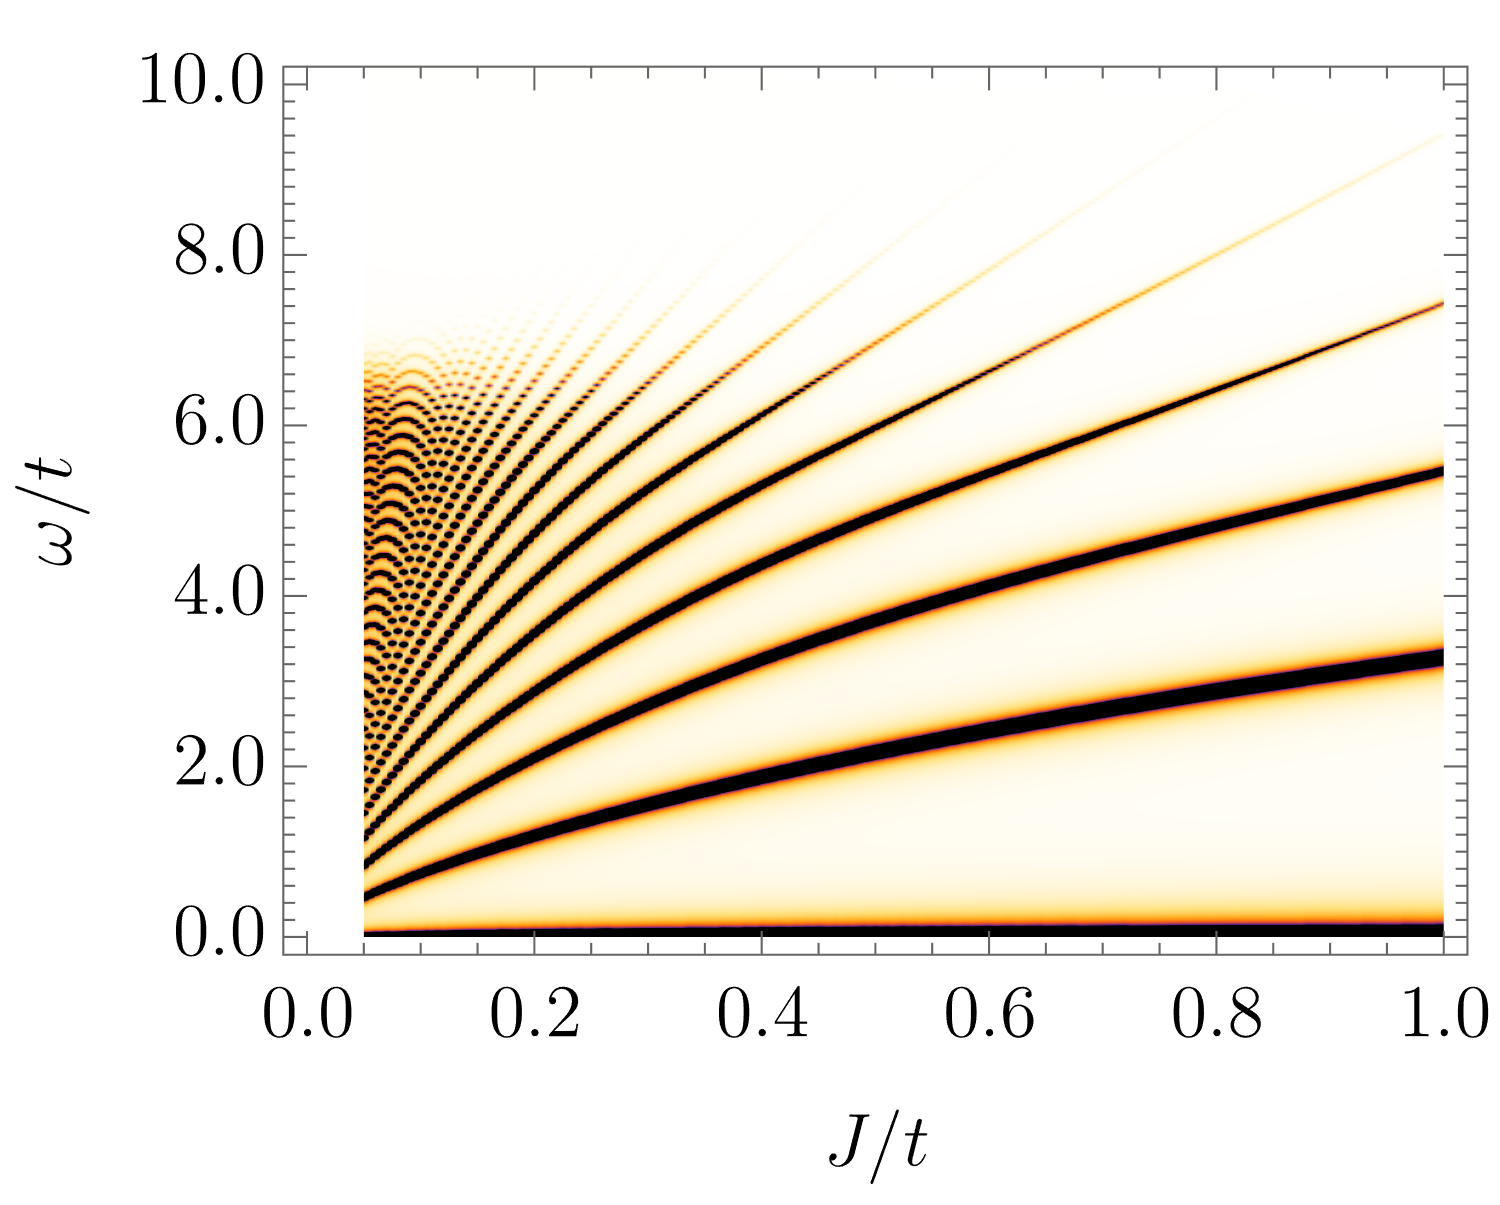
\includegraphics[width=0.79\columnwidth]
	{./figures/bethe.png}
	\caption{
		Single hole in a Bethe lattice. The spectral function $A(\omega)$ for $H$ without magnon interactions.
	}\label{fig:no_crossing}
\end{figure}

\begin{figure}[h!]
	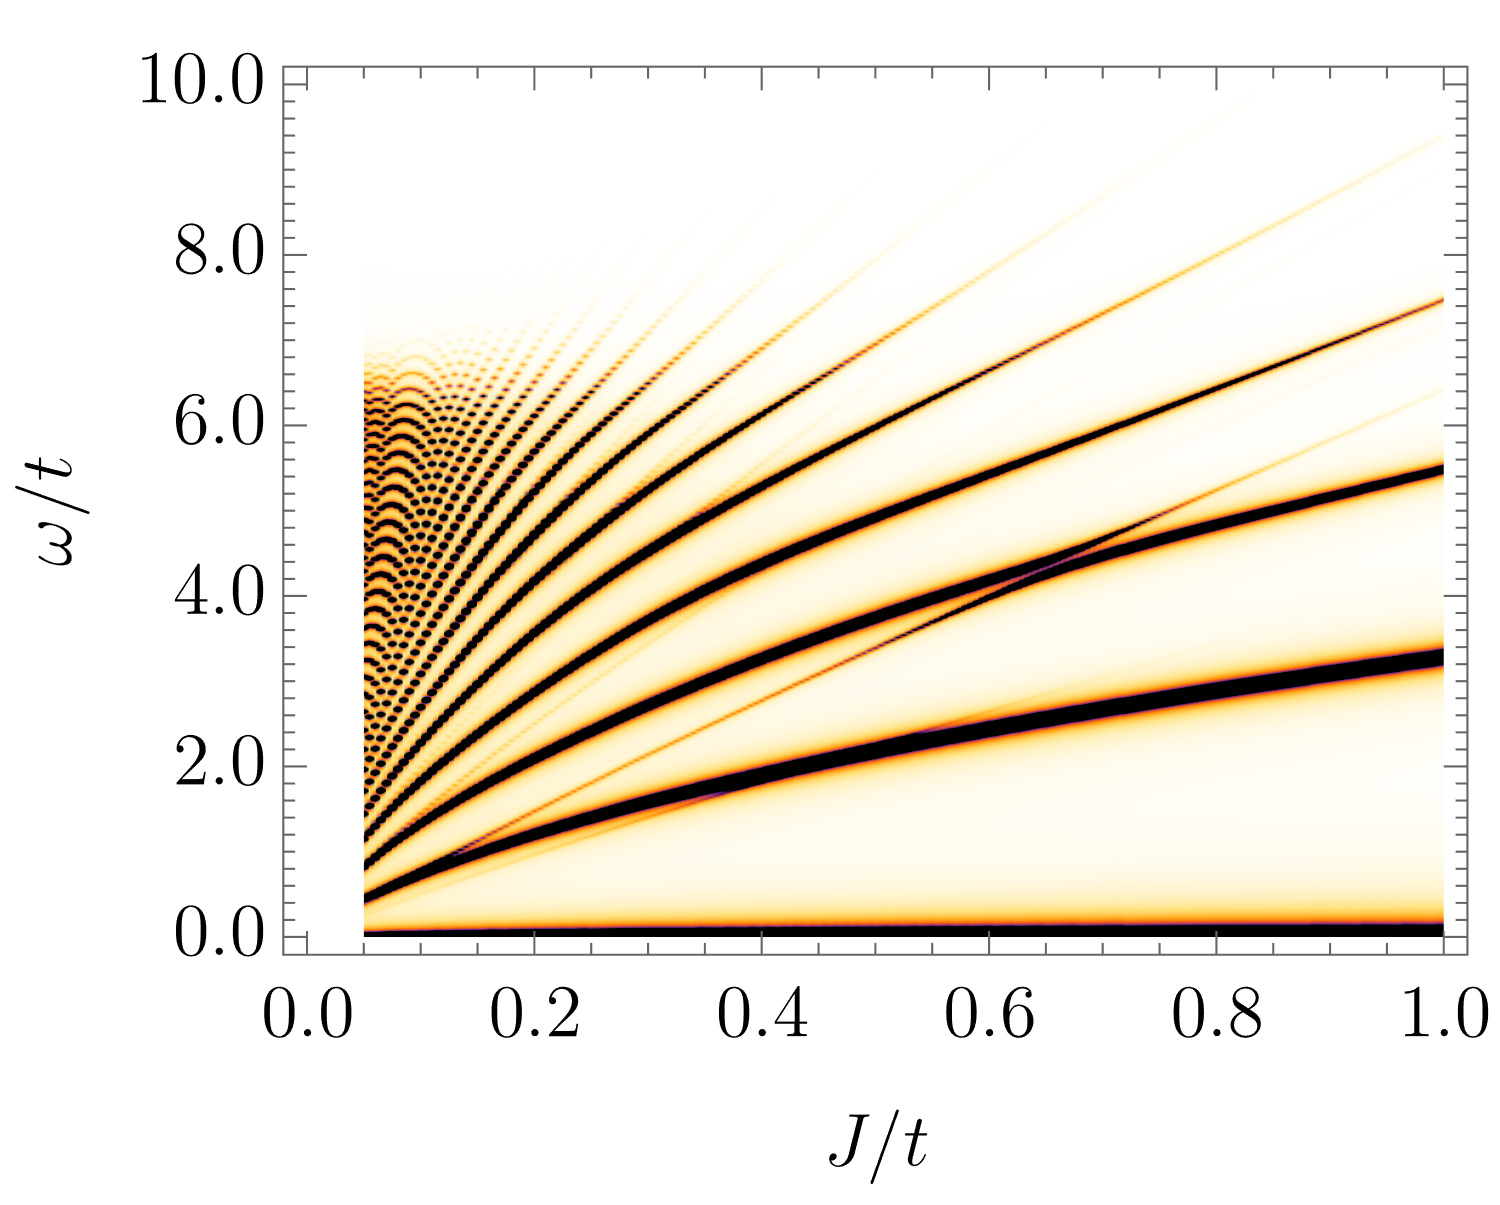
\includegraphics[width=0.79\columnwidth]
	{./figures/bethe_acr.png}
	\caption{
		Single hole in a Bethe lattice. The spectral function $A(\omega)$ for $H + H'$ without magnon interactions. The coupling to states with non-zero angular momentum is reflected in the mixing of zero- and non-zero-like degrees of freedom appearing as the level repulsion visible in the plot.
	}\label{fig:crossing}
\end{figure}

\clearpage

\section{Linear dependence of rotational states with non-zero angular momentum}
The noticeable fact of the lowest rotational excitations (i.e. where not all the $m^{(k)}_{s_k}$ coefficients are equal to 0) is their extremally close to linear in $J/t$ splitting from the ground state. Moreover, this linear splitting seems to be related to the cost of consecutive magnons created by the moving hole. For example, in the model omitting the magnon interactions, each magnon costs the energy of $2J$. At the same time in Fig.~\ref{fig:crossing} we can observe linear states with scaling close to $4J$, $6J$ and $10J$---which corresponds to the cost of 2, 3 and 5 magnons respectively.

Let us understand in quite some detail where the above-mentioned phenomenon originates from. In the beginning, let's see how the Hamiltonian $H$ acts on the following states $\ket{n;0,...,0,0}$ and $\ket{n;0,...,0,1}$. To simplify equations let's consider $n>1$, but remember the same logic applies also for $n = 1$.
\begin{equation}
\begin{aligned}
	H\ket{n;0,...,0,0} &= E_n \ket{n;0,...,0,0} \\
	&-t\sqrt{3}\left(\ket{n-1;0,...,0} + \ket{n+1;0,...,0,0,0}\right).
\end{aligned}
\end{equation}
\begin{equation}
\begin{aligned}
	H\ket{n;0,...,0,1} &= E_n \ket{n;0,...,0,1} -t\sqrt{3}\ket{n+1;0,...,0,1,0}.
\end{aligned}
\end{equation}
When $H$ acts such that the hole annihilates the $n$-th magnon, the resulting 3 identical states $\ket{n-1;0,...,0}$ (from three paths) appear with the phase factors that sum up to 0 when the $m^{(n)}_3 \neq 0$. Therefore there is no coupling to the states with less than $n$ magnons for $m^{(n)}_3 \neq 0$. Our intuition tells us, these unremovable magnons may drive the linear shift in energy.

To further confirm the above claim, let's consider the following two Greens functions,
\begin{equation}
	G(\omega) = \bra{0}(\omega - H + E_{\varnothing})^{-1}\ket{0},
\end{equation}
which is the standard Greens function of a single hole added to the $t$--$J^z$~model, and
\begin{equation}
	G_r(\omega) =~_r\bra{1;1}(\omega - H + E_{\varnothing})^{-1}\ket{1;1}_r
\end{equation}
which is the simplest spectral function including the non-zero rotational degree of freedom. We can provide the exact expressions for both of them (for simplicity let's exclude interactions with magnons),
\begin{equation}
	G(\omega)^{-1} = G_0(\omega)^{-1} - \Sigma(\omega),
\end{equation}
where $G_0(\omega)^{-1} = \omega - 2J$ and,
\begin{equation}
	\Sigma(\omega) = \frac{4t^2}{\omega - 4J - \frac{3}{4}\Sigma(\omega - 2J)}.
\end{equation}
At the same time,
\begin{equation}
\begin{aligned}
	G_r(\omega)^{-1} 
	&= G_0(\omega - 2J)^{-1} - \frac{3}{4}\Sigma(\omega - 2J) \\
	&= G(\omega - 2J)^{-1} + \frac{1}{4}\Sigma(\omega - 2J).
\end{aligned}
\end{equation}
Notice how equations for $G(\omega)$ and $G_r(\omega)$ differ by a shift by $2J$ and some fraction of the self-energy. If we modified the geometry of the Bethe lattice only around the origin such that at this single point the coordination would be $z_0 = 3$, then we would obtain,
\begin{equation}
	G_r(\omega)^{-1} = G(\omega - 2J)^{-1}.	
\end{equation}
Therefore $G_r(\omega)$ would have the same peaks as $G(\omega)$ but shifted by $2J$---which is the cost of a single magnon that cannot be annihilated by the hole. This situation is presented in Fig.~\ref{fig:perfect_linear}. In detail, the reality is a little bit more complicated. When we consider the actual Bethe lattice, i.e. $z_0 = z = 4$, the hole has 4 branches (instead of 3) at the origin to delocalize and lower its energy. This pushes the ground state down in energy compared to the $z_0=3$ case. For this reason, the shift is not perfectly equal to $2J$. Moreover, the dependence of the ``linear" peak is also not completely linear in $J$. But the differences are small, which is shown in Fig.~\ref{fig:linear}. The same scheme generalizes to higher rotational degrees of freedom. This explains the observed close-to-linear dependence in $J/t$---it scales with the cost of the chain of magnons unremovable by the hole due to non-zero angular momenta, where a small discrepancy appears due to an imbalance in the kinetic energy of the hole at the origin compared to the other sites.

\clearpage

\begin{figure}[h!]
	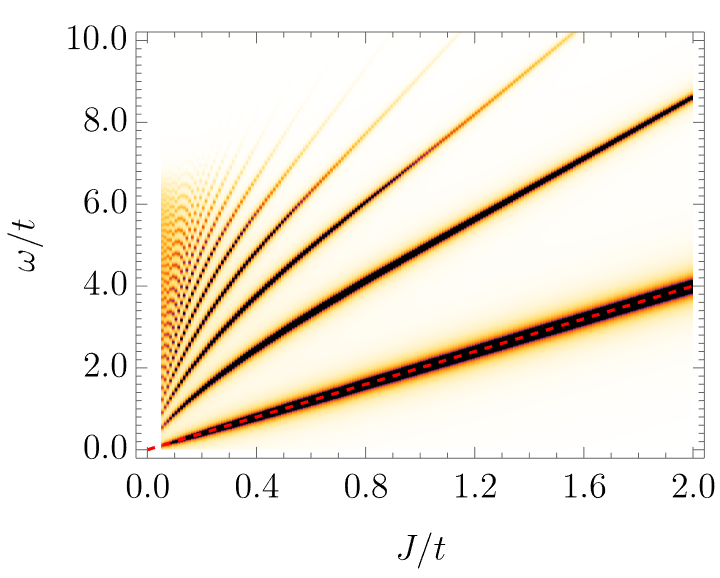
\includegraphics[width=0.73\columnwidth]
	{./figures/perfect_linear.png}
	\caption{
		Spectral function $A_r(\omega) = -\frac{1}{\pi}\lim_{\delta \to 0^+}\mathrm{Im}(G_r(\omega + i\delta))$ aligned with respect to the ground state of the $t$--$J^z$ model with a single hole on a Bethe lattice with $z = 4$ everywhere but the single point at the origin, where $z = z_0 = 3$. The dashed red line is $\omega(J) = 2J$ and it goes through the middle of the lowest rotational excitation.
	}\label{fig:perfect_linear}
\end{figure}

\begin{figure}[h!]
	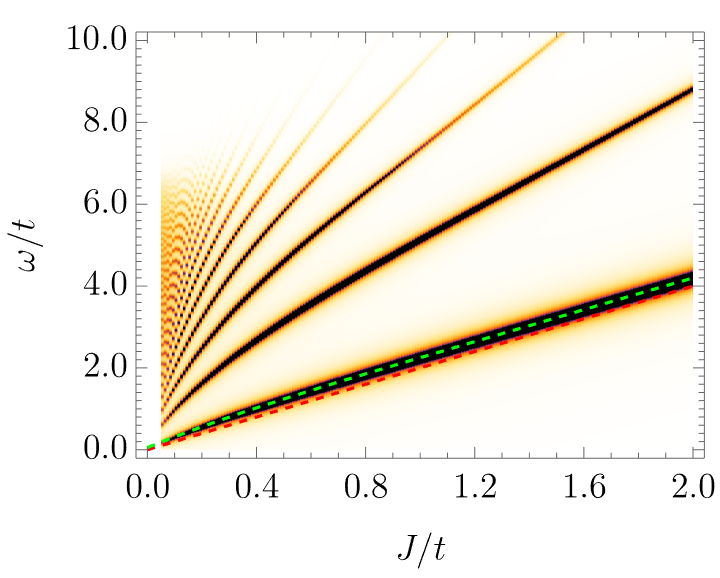
\includegraphics[width=0.73\columnwidth]
	{./figures/linear.png}
	\caption{
		Spectral function $A_r(\omega) = -\frac{1}{\pi}\lim_{\delta \to 0^+}\mathrm{Im}(G_r(\omega + i\delta))$ aligned with respect to the ground state of the $t$--$J^z$ model with a single hole on a Bethe lattice with $z = 4$ everywhere. The dashed red line is $\omega(J) = 2J$, while the dashed green line tracks the maximum of the lowest rotational excitation.
	}\label{fig:linear}
\end{figure}

\end{document}